\documentclass[]{article}
\usepackage{lmodern}
\usepackage{amssymb,amsmath}
\usepackage{ifxetex,ifluatex}
\usepackage{fixltx2e} % provides \textsubscript
\ifnum 0\ifxetex 1\fi\ifluatex 1\fi=0 % if pdftex
  \usepackage[T1]{fontenc}
  \usepackage[utf8]{inputenc}
\else % if luatex or xelatex
  \ifxetex
    \usepackage{mathspec}
  \else
    \usepackage{fontspec}
  \fi
  \defaultfontfeatures{Ligatures=TeX,Scale=MatchLowercase}
\fi
% use upquote if available, for straight quotes in verbatim environments
\IfFileExists{upquote.sty}{\usepackage{upquote}}{}
% use microtype if available
\IfFileExists{microtype.sty}{%
\usepackage{microtype}
\UseMicrotypeSet[protrusion]{basicmath} % disable protrusion for tt fonts
}{}
\usepackage[margin=1in]{geometry}
\usepackage{hyperref}
\hypersetup{unicode=true,
            pdftitle={Network based multifactorial modelling microRNA-target interaction.},
            pdfauthor={Selcen Ari; Alper Yilmaz},
            pdfborder={0 0 0},
            breaklinks=true}
\urlstyle{same}  % don't use monospace font for urls
\usepackage{graphicx,grffile}
\makeatletter
\def\maxwidth{\ifdim\Gin@nat@width>\linewidth\linewidth\else\Gin@nat@width\fi}
\def\maxheight{\ifdim\Gin@nat@height>\textheight\textheight\else\Gin@nat@height\fi}
\makeatother
% Scale images if necessary, so that they will not overflow the page
% margins by default, and it is still possible to overwrite the defaults
% using explicit options in \includegraphics[width, height, ...]{}
\setkeys{Gin}{width=\maxwidth,height=\maxheight,keepaspectratio}
\IfFileExists{parskip.sty}{%
\usepackage{parskip}
}{% else
\setlength{\parindent}{0pt}
\setlength{\parskip}{6pt plus 2pt minus 1pt}
}
\setlength{\emergencystretch}{3em}  % prevent overfull lines
\providecommand{\tightlist}{%
  \setlength{\itemsep}{0pt}\setlength{\parskip}{0pt}}
\setcounter{secnumdepth}{0}
% Redefines (sub)paragraphs to behave more like sections
\ifx\paragraph\undefined\else
\let\oldparagraph\paragraph
\renewcommand{\paragraph}[1]{\oldparagraph{#1}\mbox{}}
\fi
\ifx\subparagraph\undefined\else
\let\oldsubparagraph\subparagraph
\renewcommand{\subparagraph}[1]{\oldsubparagraph{#1}\mbox{}}
\fi

%%% Use protect on footnotes to avoid problems with footnotes in titles
\let\rmarkdownfootnote\footnote%
\def\footnote{\protect\rmarkdownfootnote}

%%% Change title format to be more compact
\usepackage{titling}

% Create subtitle command for use in maketitle
\providecommand{\subtitle}[1]{
  \posttitle{
    \begin{center}\large#1\end{center}
    }
}

\setlength{\droptitle}{-2em}

  \title{Network based multifactorial modelling microRNA-target interaction.}
    \pretitle{\vspace{\droptitle}\centering\huge}
  \posttitle{\par}
    \author{Selcen Ari\footnote{Yildiz Technical University Department of
  Bioengineering} \\ Alper Yilmaz\footnote{Yildiz Technical University Department of
  Bioengineering}}
    \preauthor{\centering\large\emph}
  \postauthor{\par}
      \predate{\centering\large\emph}
  \postdate{\par}
    \date{28 Mayıs 2019}


\begin{document}
\maketitle

\hypertarget{abstract}{%
\subsection{Abstract}\label{abstract}}

Competing endogenous RNA (ceRNA) regulations and crosstalk between
various types of non-coding RNA in human is remarkable in means of miRNA
regulation. Many studies have pointed out that an alteration in
miRNA:target interaction can result in unexpected changes due to
indirect and complex interactions. In this paper, we defined a new
network-based model that handles miRNA:ceRNA interactions with
expression values. Our model is able to handle miRNA interaction factors
such as seed type, binding energy, if provided. Our approach is able to
reveal that a perturbation in an element of network affects whole
competing elements differently and cooperative efficiencies of miRNAs on
common targets could be calculated. Our findings emphasized importance
of miRNA:target ratios being crucial, as reported by previous studies.
We have showed that the competing elements which have the same or close
expression values may not be affected equally from the perturbation
because of repression functionality depended on interaction factors of
miRNA target pairs (TOFIX: Hocam etkileşim faktörlerinden dolayı
ekspresyonları yakın olsa bile baskılanma aktitesinin aynı
sergilenmeyeceğini ifade etmeye çalıştım. Bu şekilde anlaşılıyor mu?).
We applied the model to real sample consisting of breast cancer gene and
miRNA expression dataset and experimental miRNA:target interaction
dataset all generated via high throughput sequencing methods. A gene
over-expressed in tumor tissue, namely \emph{ABCC1}, is used as
perturbing element. We have observed that change in expression level of
single gene in miRNA:target network is sufficient to perturb regulations
in whole network, due to unforeseen and unpredicted regulation which are
only visible when considered in network context. Therefore, this model
helps unveiling the crosstalk between elements in miRNA:target network
where abundance of target and sponge effect are taken into account. The
model is scalable and can be plugged in with emerging miRNA effectors
such as circRNAs. The model is available as R package at
\url{https://github.com/selcenari/ceRNAnetsim}. (TODO the link will
change)

\hypertarget{introduction}{%
\subsection{Introduction}\label{introduction}}

MicroRNAs (miRNAs) are a family of short non-coding RNAs which are key
regulator of gene expression through various post-transcriptional
mechanisms. Although the mechanisms by which miRNA represses are not
fully understood, miRNAs predominantly repress their targets. Repressive
activities of miRNAs vary depending on many factors that are significant
to microRNA:target interactions. These factors include microRNA:target
binding energy, binding location in target sequence, base pairing types
between miRNA and target, abundance of miRNAs and targets (Grimson et
al. 2007). Binding energies of miRNA:target complexes vary based on
nucleotide context and determine folding stability of complex (Cao and
Chen 2012). It has been demonstrated that the binding energy between
miRNA and target indicates stability or affinity of complex (Helwak et
al. 2013) and does not directly determine repressive activity of miRNA
(Cao and Chen 2012). Early studies have argued that 2-8 nt sequence,
seed, located in miRNA 5'end bind to specific sequence located in 3'UTR
of its target (Bartel 2004; Lewis, Burge, and Bartel 2005). In recent
studies, it has been shown that miRNAs can interact with targets via
sequences located in regions such as 5'UTR or CDS (Hausser et al. 2013;
Helwak et al. 2013; Moore et al. 2015). These studies also showed that
binding location could indicate functionality of miRNA:target
interaction or be effective on abundance of targets(TOFIX abundance
etkisi derken, bazen azaltabilir, bazen arttırabilir, manasında mı?,
evet hocam anlaşılmıyorsa değiştirebilirim). It has been shown that
miRNAs exhibit repressive activity via, 6-8 nt long sequence that is
perfectly complementary with targets, seed region at the 5' end of
miRNAs (Bartel 2009; Grimson et al. 2007). On the other hand, some
researchers have reported that seed sequence of miRNA can have
mismatches or bulged/wobble nucleotides and may locate in region other
than 5'end of miRNAs (Hafner et al. 2010; Helwak et al. 2013). On top of
all these factors, abundance of miRNAs and targets and miRNA:target
ratio in cells predominantly affect efficiency of miRNA:target
interaction (Arvey et al. 2010; Bosson, Zamudio, and Sharp 2014; Denzler
et al. 2014).

As it is possible for miRNAs to suppress multiple targets, an individual
mRNA molecule can also be targeted by multiple miRNAs. In that case, the
targeted mRNAs exhibit competitor behavior, that is hypothesized as
competing endogenous RNAs (ceRNAs) (Ala et al. 2013; Cesana and Daley
2013), against their miRNAs. Briefly, Ala et al.~have explained the
ceRNA hypothesis as disturbance of the other target when one of the
targets on a steady-state system that included one miRNA and two target
was perturbed with expression change (Ala et al. 2013). Regarding
interaction between miRNAs and their target in a cell, explaining and
predicting results of an individual perturbation is difficult due to
complexity of interactions. Various computational and experimental
studies have tackled the problem of unraveling ceRNA:miRNA interactions.
It has been observed that when abundance of one of the targets of
miR-122 was increased, the other target expression also slightly
increased as a result of decreasing repressive activity of miR-122 on
them (Denzler et al. 2014). Bosson et al.~have developed a mathematical
model for changes on total target pool concentration after grouping
targets according to affinity and demonstrated that miRNA activity
correlated with affinity between miRNA and target (Bosson, Zamudio, and
Sharp 2014). Cooperative efficiency of miRNAs as well as competitor
behaviors of targets were also studied and it has been demonstrated to
be crucial for regulating available mRNA levels of targets (Denzler et
al. 2016). MiRNA:target interactions have been modeled as stoichiometric
and catalytic mechanisms and Figliuzzi et al.~have recommended handling
models in network context (Figliuzzi, Marinari, and De Martino 2013).
The model that can explain miRNA target interaction through topological
features has been applied at bipartite network by Nitzan et al.~(Nitzan
et al. 2014). Robinson and Henderson applied the model that handles
miRNA:target direct and indirect interactions via common miRNA of gene
and target of miRNA, at bipartite network. It has been demonstrated that
all miRNAs and targets in the network can interact with each other
through common miRNAs and genes, without interaction between the same
type of nodes (Robinson and Henderson 2018).Associated genes that are
targets of the same miRNAs have been found with help of correlation of
gene expression changes in recent algoritm (Markus List 2017). List et
al.~have specified that their approach can be useful for ceRNA studies
and published their approach as an R package.

\hypertarget{methods}{%
\subsection{Methods}\label{methods}}

\hypertarget{mirnatarget-ratio-theoretical-action-in-network-based-cerna-model}{%
\subsubsection{miRNA:target ratio theoretical action in network based
ceRNA
model}\label{mirnatarget-ratio-theoretical-action-in-network-based-cerna-model}}

We developed a novel network based approach that can use to simulation
of gene regulation after any perturbation at miRNA:target interactions.
If a perturbation or change induces on graph, whole interacted nodes
vary because of changes in miRNA:target ratios. The system was assumed
as steady state that miRNAs affect according to the ratio of the
individual target to all targets (\autoref{fig1}a, expression values
shown as integer for comprehensible sampling). When expression of gene 2
(G2) increased to two fold (\autoref{fig1}b), distribution of miRNA (M1)
expression changes (\autoref{fig1}c). Consequently, expression of common
target (G4) of miRNA1 and miRNA2 also varies. The change at expression
of common target triggers to changes of proportional distribution of
miRNA2 (\autoref{fig1}d).

\begin{figure}
\hypertarget{fig1}{%
\centering
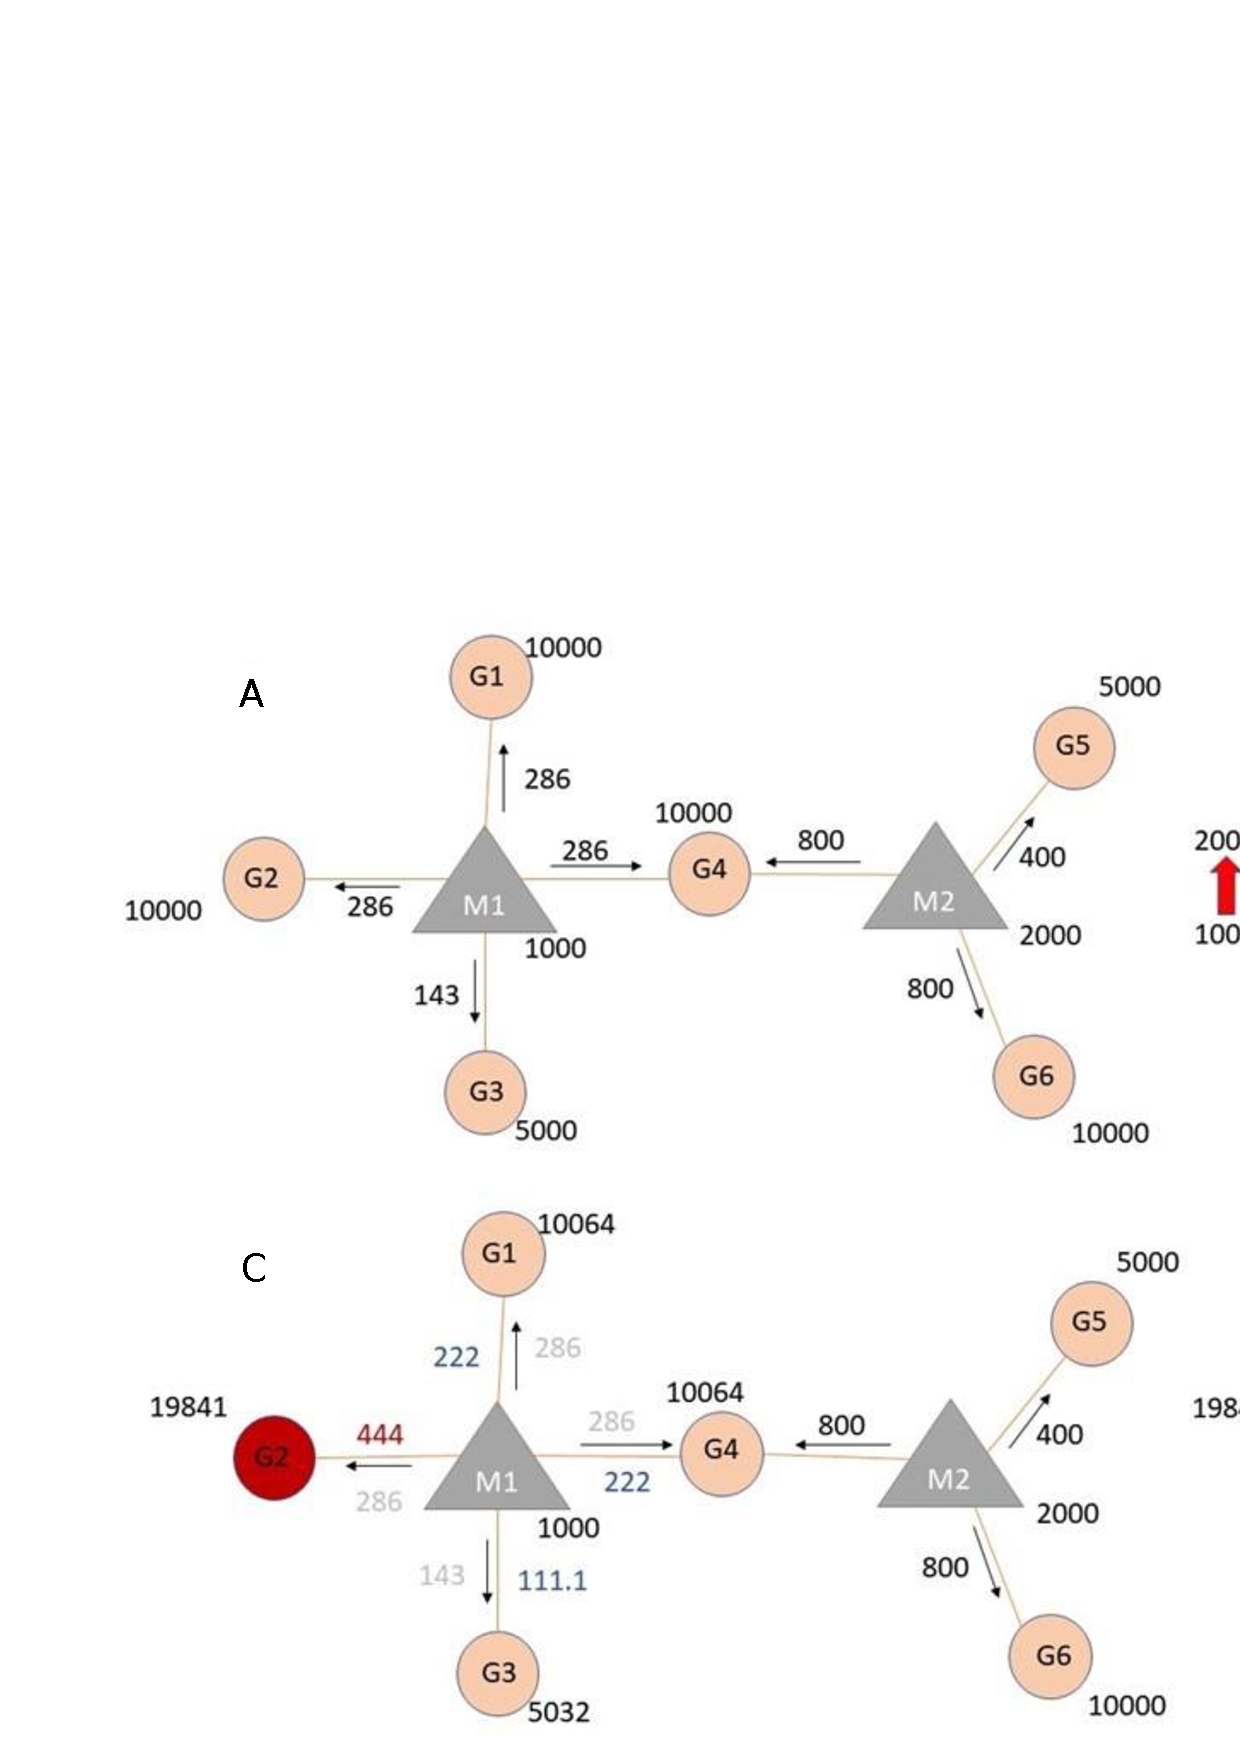
\includegraphics{Fig1.jpg}
\caption{Schematic presentation of mechanism of network based model. a)
In steady state, miRNAs (M: gray triangle) repress targets (G: circle
coconut) according to proportion of their targets' expression. b-c-d)
MiRNA expression distributions to targets vary when expression of one of
the targets perturbed.}\label{fig1}
}
\end{figure}

The model was developed by making some assumptions. Transcription rates
and degradation rates of miRNAs were assumed as stationary and equal.
Targets also have stable transcription and degradation rates, at the
same time they are equal. The factors that could be affect the
miRNA:target interaction are disregarded in this approach. It is
considered that miRNAs degrades or inhibits them via any mechanisms
after binding to target while the miRNAs were used reversibly. In
initial conditions, gene expression amounts in system have been
considered after repression activity of miRNAs. If a change occurs in
the system, variation on miRNA proportional distribution are reflected
as change of repression activity. \begin{equation} 
    Eff_{gi}= C_m * C_{gi}/\sum_{1}^{i} C_g \tag{1}\label{eq:1}
\end{equation} \begin{equation}
   R_{gi}= Eff_{i1}+ Eff_{i2} ... \tag{2}\label{eq:2}
\end{equation}

The efficiency of a miRNA on the individual target (\(Eff_{gi}\)) is
calculated according to equation \eqref{eq:1}; \(C_m\), miRNA expression
in the group; \(C_{gi}\), symbolize individual gene expression; \(C_g\)
gene expressions in the group (Groups are determined depending on
miRNAs. Targets that are interacted with the same miRNA find in a
group.). In this approach, because a gene can be found in different
groups, the cooperative activity of microRNAs also can be calculated.
Total repression activity of different miRNAs on the common target,
\(R\), is calculated based on equation \eqref{eq:2}; sum of efficiency
of different miRNAs on the target.

\begin{figure}
\hypertarget{fig2}{%
\centering
\includegraphics{fig2.jpg}
\caption{Calculations to determine of miRNA binding and repression
efficiency. \(G\), Gene; \(M\), miRNA; \(STE\), seed type effect;
\(RE\), Region Effect; \(E\), Energy; \(STE’\), normalized values of
seed type efficiency coefficient; \(RE’\), normalized values of region
efficiency coefficient; \(E’\), normalized values of energy
coefficient.}\label{fig2}
}
\end{figure}

\hypertarget{mirna-action-in-network-based-multifactorial-cerna-model}{%
\subsubsection{miRNA action in network based multifactorial ceRNA
model}\label{mirna-action-in-network-based-multifactorial-cerna-model}}

Interactions between miRNAs and their targets can be affected from
different parameters. For this reason, we improved model with factors
that can affect to miRNA activity. In our approach, the parameters are
classified as binding and efficiency factors and all of these are
evaluated in their groups. Binding factors determine interaction between
miRNA and target. The efficiency factors decide functionality of
binding. In the literature, binding free energy (Cao and Chen 2012 ;
Helwak et al. 2013) and seed type (Werfel et al. 2017) in miRNA:target
interactions are represented as binding affinity. Efficiency factors
determine how many of microRNA:target complexes will result in
inhibition. For example, binding region on the target shows whether the
target can be inhibited (functionality)(Hausser et al. 2013; Helwak et
al. 2013). Both of binding and efficiency factors are evaluated in the
groups and normalized according to equation \eqref{eq:3}; each factor is
normalized based on maximum variables that found in their groups.
\begin{equation}
F`= F/F_{max} \tag{3}\label{eq:3}
\end{equation}

The normalized values of factors take into account to determine binding
activity and miRNA efficiency on targets (\autoref{fig2}). Binding
affinities (activity, \(Eff\)) of miRNAs on each individual gene are
calculated as shown in equation \eqref{eq:4}; \(C_m\), miRNA expression
in the group; \(C_g\), Gene expression; \(C_{gi}\), individual gene
expression; gi, individual gene; g, whole genes in a group
(\autoref{fig2}c). \begin{equation}
Eff_{gi}= C_m * E`_{gi}*STE`_{gi}*C_{gi}/(\sum_{1}^{i} E`_{gi}*STE`_{gi}*C_{gi}) \tag{4}\label{eq:4}
\end{equation} \begin{equation}
Eff_{gi}= Eff_{gi}*RE`_{gi} \tag{5}\label{eq:5}
\end{equation}

After miRNA binds to its target, but might not repress to bound target.
The functionality of bound miRNA on target depends on efficiency factors
like region that is binding sequence of miRNA on its target. Exact
repression efficiency of miRNA is calculated according to equation
\eqref{eq:5} (\autoref{fig2}d); \(RE’_{gi}\), normalized values of
region efficiency coefficient between miRNA and gene. The cooperative
repression activity of miRNAs to their common targets is figured out as
shown in \autoref{fig2}e.

\hypertarget{application-of-model-in-a-breast-cancer-patient-dataset}{%
\subsubsection{Application of model in a breast cancer patient
dataset}\label{application-of-model-in-a-breast-cancer-patient-dataset}}

To determine suitability of method, we have tried to apply model in a
real dataset. Firstly, we obtained the miRNA and gene expression
datasets of the patient's tumor and normal tissue. We downloaded the
high-throughput experimental datasets which are provided miRNA:gene
target pairs with interaction factors by
\textbf{moore\_mirnatarget\_2015} and (Helwak et al. 2013). We have
combined miRNA and gene expression datasets via miRNA:target gene
dataset \textbf{(Whole steps can be found in Supplementary
data(TCGA\_E9-A1N5\_article.Rmd)}). We selected a gene which is over
expressed in tumor tissue with compared to normal tissue. It is pointed
out that ABCC1 gene, \emph{Multidrug resistance-associated protein 1},
is one of the most significant factor to develop resistance against
chemotherapotic agents(Atalay, Demirkazik, and Gunduz 2008; Lu et al.
2015; Atalay et al. 2006). So, we selected ABCC1 gene for simulation of
integrated dataset. We have detected the iteration that is suitable for
ABCC1 gene simulation. After simulation of system via ABCC1 gene with
over expression, we have compared simulation results and tumor tissue
expression levels.

\hypertarget{results-and-conclusions}{%
\subsection{Results and Conclusions}\label{results-and-conclusions}}

We have developed a model approach and workflow for competitive ceRNA
regulation in this study. The basic mode of miRNA repression activity
has been based on miRNA and target abundance in various researches(Arvey
et al. 2010; Denzler et al. 2014). For this reason, we performed first
application as considering only abundance of miRNAs and targets
(\autoref{fig1}). After the increasing in a gene expression value,
expression values of other genes also changed slightly in comparison
with alteration in perturbation started gene node. Different studies
have shown that the other gene expression values also rise differently,
if a gene abundance increases in ceRNA system (Lai, Wolkenhauer, and
Vera 2016; Salmena et al. 2011; Tay, Rinn, and Pandolfi 2014). It was
observed that primary neighborhoods of the trigger gene change with the
same ratio, but cooperative efficiency of miRNAs on common target causes
differently change in common target (\autoref{fig1}d). The common target
in system has displayed like a trigger for the other group and induced
changes of expression values of genes on the other group. Therefore,
effect of primary change of the gene (G2) on genes of the other group
was observed slightly (\autoref{fig1}d). In addition, like shown by
ceRNA hypothesis model of Ala et al., after the increasing of a gene
expression (G2), the miRNA that is found in the same group (M1) tended
to be more repressive on this target. This has caused to decrease in
increased expression value of primer triggering gene. When the
expression of a gene (G2) was increased to two fold, we observed that
the expression changes were more evident. So, we have considered that
high miRNA:target ratio results in stronger miRNA repression activity.
This results also are coherent with previous reports that were offered
by Arvey et al.~and Denzler et al.(Arvey et al. 2010; Bosson, Zamudio,
and Sharp 2014; Denzler et al. 2014). When the simulation was run in
sample dataset that includes lower target abundance, the first response
of primary neighborhood of the same group was determined as similar with
in system that have high target abundance. But regulations of ceRNAs
were observed differences in the following steps of simulation. In
overall state in the end of simulation, we have established that all
regulations more prominent when compared with low miRNA:target ratio
dataset. The model has appeared the importance of mRNA:target ratio in
regulation of competing RNAs.

\begin{figure}
\hypertarget{fig3}{%
\centering
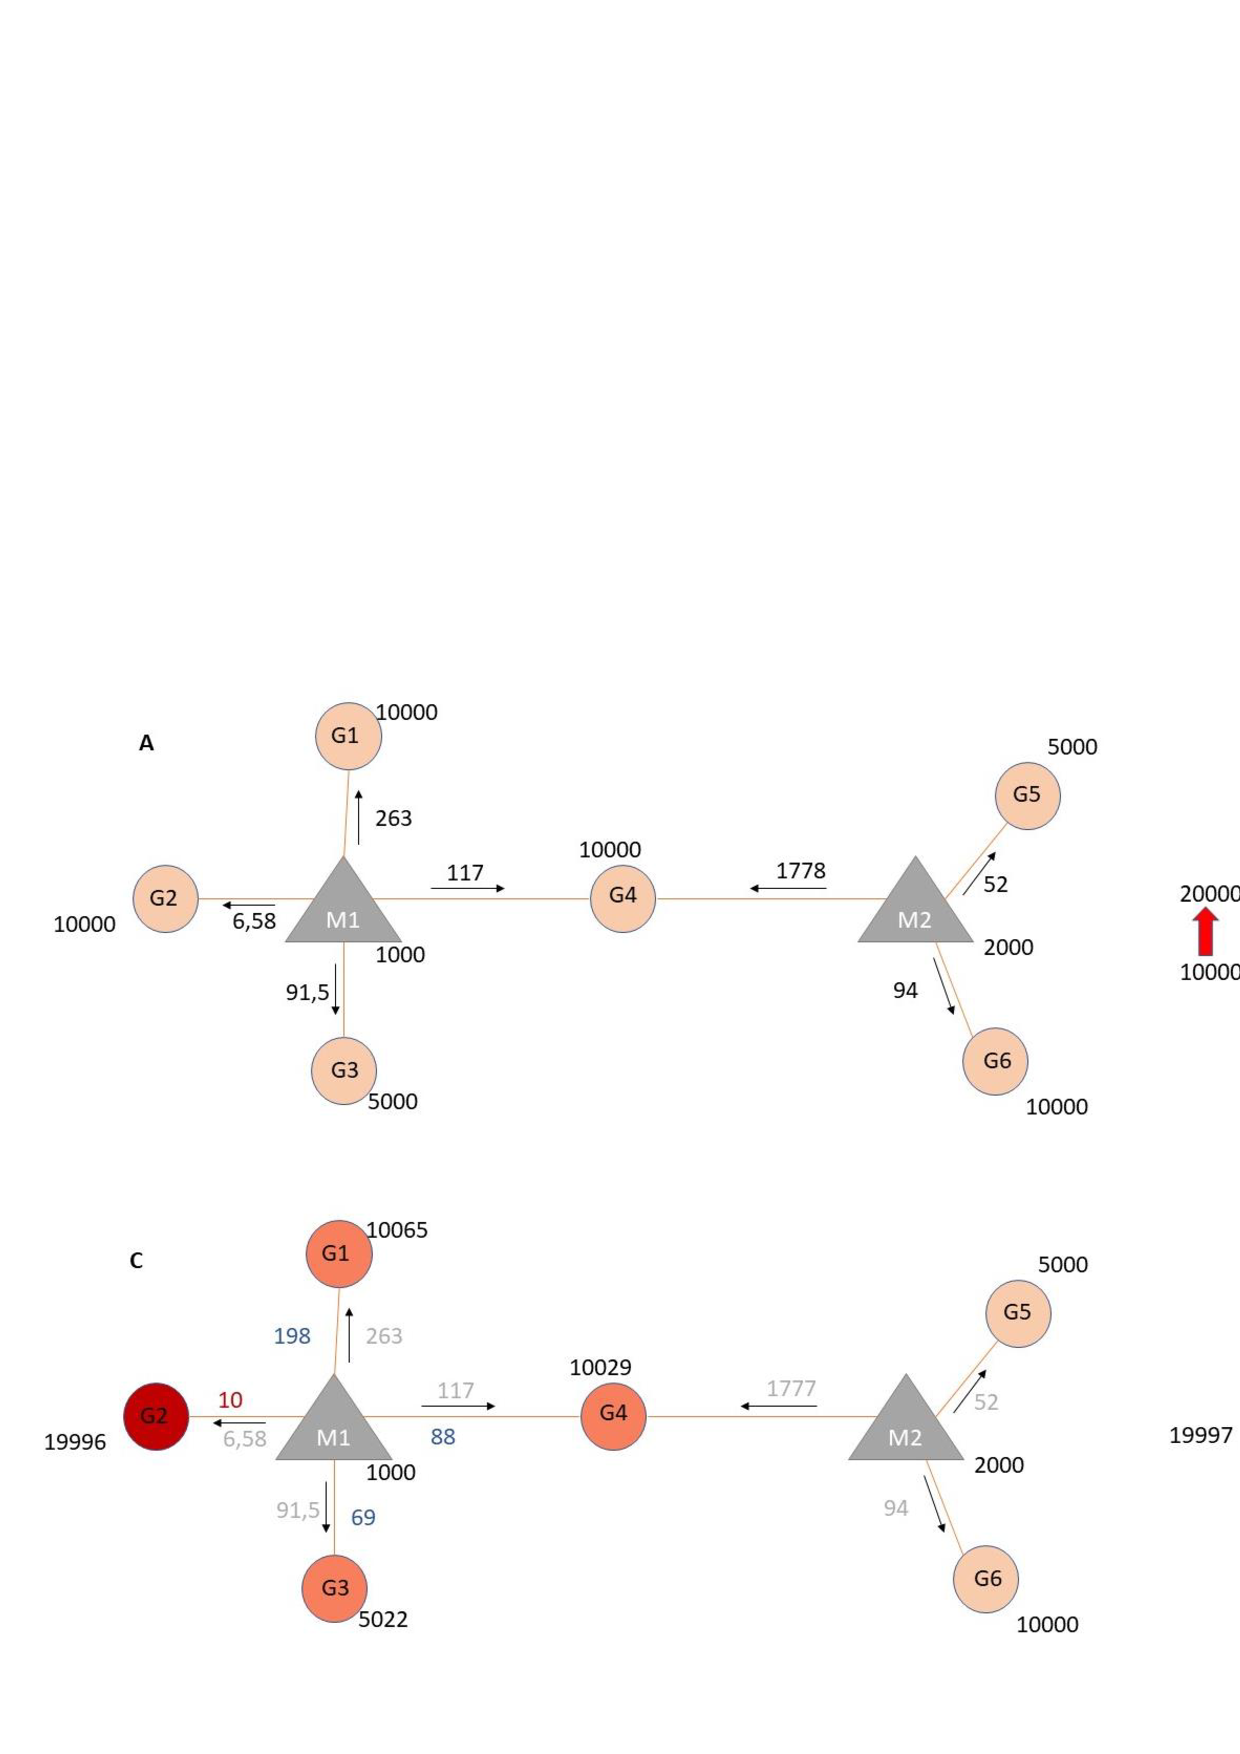
\includegraphics{Fig3.jpg}
\caption{Target regulations with interaction parameters. a) In the
steady-state the repression activity of miRNAs on the targets after
binding and repression efficiency. b) The changes the repression
activities after increasing of G2 expression. c) Perturbation of primary
neighborhoods of M1 miRNA (M1 miRNA group). d) Regulation of gene
expression of other gene group via triggering target (common target
between M1 and M2).}\label{fig3}
}
\end{figure}

It has been reported in several studies that miRNA regulatory
interactions also is affected different parameters. For example, Xu et.
al have investigated the importance of seed pairing type between miRNAs
and their targets and target site location by using proteomics dataset
(Xu, Wang, and Liu 2014). They have proposed that the features of
binding between miRNA and target can be critical efficiency of miRNA and
can be used to find effective miRNA molecules. In addition, binding
energy between miRNA and targets also could be determinant for miRNA
efficiency. It has been reported by Breda et. al.~that strength of
miRNA:target interactions is depended on binding energy of complexes
(Breda et al. 2015). As similar to these, Bosson et al.~have associated
affinity and seed pairing of miRNA target pairs and suggested that
number of canonical base pairing is correlated with affinity. For these
reasons, we have improved the model with optional interaction parameters
that could be useful for understanding of miRNA repression activity. We
have explained the model in the same sample dataset with using different
factors and simulated via the same change (\autoref{fig3}). When the
factors were taken into account in the system, miRNA efficiencies varied
as shown in \autoref{fig3}a. Although the miRNA target ratios in initial
states were same in comparison with the sample dataset without factors,
efficiency of binding and repression have changed. When expression of a
gene (G2) increased, expression values of all genes also change
differentially because of contribution of efficiency factors
(\autoref{fig3} b,c,d). We have considered that in our approach energy
and seed type of pairs is significant for binding and targeted region is
important for repression. But these factors can be handled optionally
and differently.

In regulation of miRNA target sample system (\autoref{fig3}), miRNA (M1)
repressive efficiency on the primary triggering gene (G2) is low in
steady-state. So it has been observed that the regulatory activities of
miRNA efficiencies on the targets are weak after the increase of miRNA
target G2. When we ran to model with two fold increasing expression
value of common target (G4), the changes of other gene expressions have
observed more prominent. Furthermore, folding of expression of target
gene that has strong miRNA repression efficiency also resulted in
evident perturbation. On the other hand, It was observed that Gene2 was
weakly affected from change of Gene4 expression because of its weak
interaction factors.This also shows that the perturbation-initiation
element in the system is important parameter. So, we also have developed
an approach that is found perturbation efficiencies of elements in
dataset. \textbf{(see details in Supplementary File(fig1\_2app.Rmd)}.
When we applied the method on the minimal dataset, while Gene4 is the
most efficient element in terms of number of perturbed elements, it have
observed that Mir2 is most potent element in the mean of expression
change. In our approach, the elements behave differently based on type
(competing or miRNA). When a competing element was changed, whole
elements out of miRNAs are re-regulated. But, if a miRNA was perturbed,
whole competing elements are re-regulated and miRNA preserves expression
at after perturbation.

The defined miRNA' number is very low in comparison with defined protein
coding genes' number. So, this results in that the miRNA amounts in the
system must be high or targeted RNAs' amount must be low for effective
miRNA activity. We have tried to simulate a real dataset which contains
thousands of genes and hundreds of miRNAs. Firstly, we have observed the
activities in the iterations and determined behaviors of the network
after simulation. As expected, we have observed that the big dataset,
compared to those containing a few genes and miRNAs, exhibited
cumbersome behaviors and complexity to gain steady-state \textbf{(see
details in Supplementary File(TCGA\_E9-A1N5\_article.Rmd)}. We realized
that a small change in a system with a large change actually brought
many arrangements. This can be explained with the competing groups.
Because the genes are targeted with many common miRNAs, and this results
in that the common targets exhibit competing behaviors in different
groups. On the other hand, the changes of gene expressions were very
different. While the change in some of genes were highly evident, some
have changed slightly. So, we have compared two datasets; the tumor gene
expression and simulation results. When we analyzed comparison of two
datasets, we have observed that the results of simulation is not
convenient with tumor tissue expression values. The simulation results
were not expected to be concordant with tumor tissue expression values
because of a single gene could not be responsible for gene regulation in
all tissue. Besides, the all other factors such as up/down regulation of
miRNAs or other genes were ignored. Of course, it would be more useful
to test a dataset that includes gene expression values before and after
the regulation of a gene and miRNA expression values at initial
conditions. When we evaluated the suitability of approach, the approach
allows different miRNA targets to be considered together and can work
with different regulatory elements due to the network structure.

The network based approaches have been developed in previous studies.
Figliuzzi et al.~have tried to explain the ceRNA crosstalk in a
network-like minimal interaction structure with concentrations of ceRNA
and miRNAs. They have pointed out that the larger miRNA number can cause
to evident crosstalk between ceRNAs. It has been thought that miRNAs and
their targets interactions depend on rates of transcription,
degradation, binding and unbinding in the network based kinetic model
which has been developed by Nitzan et al.~Nitzan and collaborators have
used the high throughput experimental dataset (Helwak et al. 2013) for
miRNA:target pair that occur high free energy and microarray dataset of
a miR-92a depletion for expression values. They have been demonstrated
that distant ceRNAs can interact with each other via indirect links, and
the interactions change to depend on distance between ceRNAs, and
topological features of network (Nitzan et al. 2014). List et al.~have
developed an approach to detect ceRNA interaction by using the miRNA
expression, gene expression and common miRNAs between gene targets
(Markus List 2017). Their approach could be useful to analysis
interacted genes through miRNAs. When it has been thought that a miRNA
can exhibit strong functionality to a target but may not against an
other, common miRNA based approach can be inconvenient to understand
regulations of ceRNA interactions.

In our approach, we have not taken into account transcription,
degradation or binding rates of elements in network. Because, although
it is known as the miRNAs are highly stable, the transcription and
degradation rates of miRNAs change to depend on according to cellular
conditions (Rüegger and Großhans 2012). According to our search, there
is no dataset that was includes to degradation and transcription rates
on specific cellular conditions for each miRNA. So, we preferred to
accept that degradation and transcription rates of each miRNAs are equal
to each other, instead of determining a constant value for all miRNAs in
the system (The same applies to mRNA.). On the other hand other
regulation parameters such as gene-gene interactions and transcription
factors are ignored but the network structure can promote to integration
of other regulation elements. In the future, with development in
experimental techniques about features of miRNAs and their targets, more
consistent and useful results can be obtained from our approach.
Additionally, this can provide to contribution to prediction of abnormal
regulations and pathways with the studies that will be developed.

\hypertarget{references}{%
\subsection*{References}\label{references}}
\addcontentsline{toc}{subsection}{References}

\hypertarget{refs}{}
\leavevmode\hypertarget{ref-ala_integrated_2013}{}%
Ala, U., F. A. Karreth, C. Bosia, A. Pagnani, R. Taulli, V. Leopold, Y.
Tay, P. Provero, R. Zecchina, and P. P. Pandolfi. 2013. ``Integrated
Transcriptional and Competitive Endogenous RNA Networks Are
Cross-Regulated in Permissive Molecular Environments.''
\emph{Proceedings of the National Academy of Sciences} 110 (18):
7154--9. \url{https://doi.org/10.1073/pnas.1222509110}.

\leavevmode\hypertarget{ref-arvey_target_2010}{}%
Arvey, Aaron, Erik Larsson, Chris Sander, Christina S Leslie, and Debora
S Marks. 2010. ``Target mRNA Abundance Dilutes microRNA and siRNA
Activity.'' \emph{Molecular Systems Biology} 6 (April).
\url{https://doi.org/10.1038/msb.2010.24}.

\leavevmode\hypertarget{ref-atalay2006multidrug}{}%
Atalay, Can, Ismet Deliloglu Gurhan, Cigdem Irkkan, and Ufuk Gunduz.
2006. ``Multidrug Resistance in Locally Advanced Breast Cancer.''
\emph{Tumor Biology} 27 (6): 309--18.

\leavevmode\hypertarget{ref-atalay2008role}{}%
Atalay, C, A Demirkazik, and U Gunduz. 2008. ``Role of Abcb1 and Abcc1
Gene Induction on Survival in Locally Advanced Breast Cancer.''
\emph{Journal of Chemotherapy} 20 (6): 734--39.

\leavevmode\hypertarget{ref-bartel_micrornas_2004}{}%
Bartel, David P. 2004. ``MicroRNAs.'' \emph{Cell} 116 (2): 281--97.
\url{https://doi.org/10.1016/S0092-8674(04)00045-5}.

\leavevmode\hypertarget{ref-bartel_micrornas:_2009}{}%
Bartel, David P. 2009. ``MicroRNAs: Target Recognition and Regulatory
Functions.'' \emph{Cell} 136 (2): 215--33.
\url{https://doi.org/10.1016/j.cell.2009.01.002}.

\leavevmode\hypertarget{ref-bosson_endogenous_2014}{}%
Bosson, Andrew D., Jesse R. Zamudio, and Phillip A. Sharp. 2014.
``Endogenous miRNA and Target Concentrations Determine Susceptibility to
Potential ceRNA Competition.'' \emph{Molecular Cell} 56 (3): 347--59.
\url{https://doi.org/10.1016/j.molcel.2014.09.018}.

\leavevmode\hypertarget{ref-breda_quantifying_2015}{}%
Breda, Jeremie, Andrzej J. Rzepiela, Rafal Gumienny, Erik van Nimwegen,
and Mihaela Zavolan. 2015. ``Quantifying the Strength of miRNA--Target
Interactions.'' \emph{Methods} 85 (September): 90--99.
\url{https://doi.org/10.1016/j.ymeth.2015.04.012}.

\leavevmode\hypertarget{ref-cao_predicting_2012}{}%
Cao, Song, and Shi-Jie Chen. 2012. ``Predicting Kissing Interactions in
microRNA--Target Complex and Assessment of microRNA Activity.''
\emph{Nucleic Acids Research} 40 (10): 4681--90.
\url{https://doi.org/10.1093/nar/gks052}.

\leavevmode\hypertarget{ref-cesana_deciphering_2013}{}%
Cesana, Marcella, and George Q. Daley. 2013. ``Deciphering the Rules of
ceRNA Networks.'' \emph{Proceedings of the National Academy of Sciences
of the United States of America} 110 (18): 7112--3.
\url{https://doi.org/10.1073/pnas.1305322110}.

\leavevmode\hypertarget{ref-denzler_assessing_2014}{}%
Denzler, Rémy, Vikram Agarwal, Joanna Stefano, David P. Bartel, and
Markus Stoffel. 2014. ``Assessing the ceRNA Hypothesis with Quantitative
Measurements of miRNA and Target Abundance.'' \emph{Molecular Cell} 54
(5): 766--76. \url{https://doi.org/10.1016/j.molcel.2014.03.045}.

\leavevmode\hypertarget{ref-denzler_impact_2016}{}%
Denzler, Rémy, Sean E. McGeary, Alexandra C. Title, Vikram Agarwal,
David P. Bartel, and Markus Stoffel. 2016. ``Impact of MicroRNA Levels,
Target-Site Complementarity, and Cooperativity on Competing Endogenous
RNA-Regulated Gene Expression.'' \emph{Molecular Cell} 64 (3): 565--79.
\url{https://doi.org/10.1016/j.molcel.2016.09.027}.

\leavevmode\hypertarget{ref-figliuzzi_micrornas_2013}{}%
Figliuzzi, Matteo, Enzo Marinari, and Andrea De Martino. 2013.
``MicroRNAs as a Selective Channel of Communication Between Competing
RNAs: A Steady-State Theory.'' \emph{Biophysical Journal} 104 (5):
1203--13. \url{https://doi.org/10.1016/j.bpj.2013.01.012}.

\leavevmode\hypertarget{ref-grimson_microrna_2007}{}%
Grimson, Andrew, Kyle Kai-How Farh, Wendy K. Johnston, Philip
Garrett-Engele, Lee P. Lim, and David P. Bartel. 2007. ``MicroRNA
Targeting Specificity in Mammals: Determinants Beyond Seed Pairing.''
\emph{Molecular Cell} 27 (1): 91--105.
\url{https://doi.org/10.1016/j.molcel.2007.06.017}.

\leavevmode\hypertarget{ref-hafner_transcriptome-wide_2010}{}%
Hafner, Markus, Markus Landthaler, Lukas Burger, Mohsen Khorshid, Jean
Hausser, Philipp Berninger, Andrea Rothballer, et al. 2010.
``Transcriptome-Wide Identification of RNA-Binding Protein and MicroRNA
Target Sites by PAR-CLIP.'' \emph{Cell} 141 (1): 129--41.
\url{https://doi.org/10.1016/j.cell.2010.03.009}.

\leavevmode\hypertarget{ref-hausser_analysis_2013}{}%
Hausser, J., A. P. Syed, B. Bilen, and M. Zavolan. 2013. ``Analysis of
CDS-Located miRNA Target Sites Suggests That They Can Effectively
Inhibit Translation.'' \emph{Genome Research} 23 (4): 604--15.
\url{https://doi.org/10.1101/gr.139758.112}.

\leavevmode\hypertarget{ref-helwak_mapping_2013}{}%
Helwak, Aleksandra, Grzegorz Kudla, Tatiana Dudnakova, and David
Tollervey. 2013. ``Mapping the Human miRNA Interactome by CLASH Reveals
Frequent Noncanonical Binding.'' \emph{Cell} 153 (3): 654--65.
\url{https://doi.org/10.1016/j.cell.2013.03.043}.

\leavevmode\hypertarget{ref-lai_understanding_2016}{}%
Lai, Xin, Olaf Wolkenhauer, and Julio Vera. 2016. ``Understanding
microRNA-Mediated Gene Regulatory Networks Through Mathematical
Modelling.'' \emph{Nucleic Acids Research} 44 (13): 6019--35.
\url{https://doi.org/10.1093/nar/gkw550}.

\leavevmode\hypertarget{ref-lewis_conserved_2005}{}%
Lewis, Benjamin P., Christopher B. Burge, and David P. Bartel. 2005.
``Conserved Seed Pairing, Often Flanked by Adenosines, Indicates That
Thousands of Human Genes Are MicroRNA Targets.'' \emph{Cell} 120 (1):
15--20. \url{https://doi.org/10.1016/j.cell.2004.12.035}.

\leavevmode\hypertarget{ref-lu2015microrna}{}%
Lu, Lin, Fang Ju, Hui Zhao, and Xuezhen Ma. 2015. ``MicroRNA-134
Modulates Resistance to Doxorubicin in Human Breast Cancer Cells by
Downregulating Abcc1.'' \emph{Biotechnology Letters} 37 (12): 2387--94.

\leavevmode\hypertarget{ref-markus_list_sponge_2017}{}%
Markus List, Marcel Schulz. 2017. ``SPONGE.'' Bioconductor.
\url{https://doi.org/10.18129/B9.bioc.SPONGE}.

\leavevmode\hypertarget{ref-moore_mirnatarget_2015}{}%
Moore, Michael J., Troels K. H. Scheel, Joseph M. Luna, Christopher Y.
Park, John J. Fak, Eiko Nishiuchi, Charles M. Rice, and Robert B.
Darnell. 2015. ``miRNA-Target Chimeras Reveal miRNA 3'-End Pairing as a
Major Determinant of Argonaute Target Specificity.'' \emph{Nature
Communications} 6 (November): 8864.
\url{https://doi.org/10.1038/ncomms9864}.

\leavevmode\hypertarget{ref-nitzan_interactions_2014}{}%
Nitzan, Mor, Avital Steiman-Shimony, Yael Altuvia, Ofer Biham, and Hanah
Margalit. 2014. ``Interactions Between Distant ceRNAs in Regulatory
Networks.'' \emph{Biophysical Journal} 106 (10): 2254--66.
\url{https://doi.org/10.1016/j.bpj.2014.03.040}.

\leavevmode\hypertarget{ref-robinson_modelling_2018}{}%
Robinson, J. M., and W. A. Henderson. 2018. ``Modelling the Structure of
a ceRNA-Theoretical, Bipartite microRNA-mRNA Interaction Network
Regulating Intestinal Epithelial Cellular Pathways Using R
Programming.'' \emph{BMC Research Notes} 11 (1): 19.
\url{https://doi.org/10.1186/s13104-018-3126-y}.

\leavevmode\hypertarget{ref-ruegger_microrna_2012}{}%
Rüegger, Stefan, and Helge Großhans. 2012. ``MicroRNA Turnover: When,
How, and Why.'' \emph{Trends in Biochemical Sciences} 37 (10): 436--46.
\url{https://doi.org/10.1016/j.tibs.2012.07.002}.

\leavevmode\hypertarget{ref-salmena_cerna_2011}{}%
Salmena, Leonardo, Laura Poliseno, Yvonne Tay, Lev Kats, and Pier Paolo
Pandolfi. 2011. ``A ceRNA Hypothesis: The Rosetta Stone of a Hidden RNA
Language?'' \emph{Cell} 146 (3): 353--58.
\url{https://doi.org/10.1016/j.cell.2011.07.014}.

\leavevmode\hypertarget{ref-tay_multilayered_2014}{}%
Tay, Yvonne, John Rinn, and Pier Paolo Pandolfi. 2014. ``The
Multilayered Complexity of ceRNA Crosstalk and Competition.''
\emph{Nature} 505 (7483): 344--52.
\url{https://doi.org/10.1038/nature12986}.

\leavevmode\hypertarget{ref-werfel_preferential_2017}{}%
Werfel, Stanislas, Simon Leierseder, Benjamin Ruprecht, Bernhard Kuster,
and Stefan Engelhardt. 2017. ``Preferential microRNA Targeting Revealed
by in Vivo Competitive Binding and Differential Argonaute
Immunoprecipitation.'' \emph{Nucleic Acids Research} 45 (17): 10218--28.
\url{https://doi.org/10.1093/nar/gkx640}.

\leavevmode\hypertarget{ref-xu_characterization_2014}{}%
Xu, Wenlong, Zixing Wang, and Yin Liu. 2014. ``The Characterization of
microRNA-Mediated Gene Regulation as Impacted by Both Target Site
Location and Seed Match Type.'' Edited by Thomas Preiss. \emph{PLoS ONE}
9 (9): e108260. \url{https://doi.org/10.1371/journal.pone.0108260}.


\end{document}
